% \begin{document}

\usetikzlibrary{arrows.meta} % For double arrows

\chapter{KV Store with Cache}

LRU cache, or least-recently-used cache, is a finite-sized cache that evicts the
least-recently-used entry when full. Modern CPU architecture supports
multi-layer cache. Caches closer to the CPU are faster, but also smaller. Cache
is designed to take advantage of temporal locality, where recently accessed data
isgenerally likely to be re-accessed in near future.\\

Caches are also applied more broadly: CDNs (content delivery networks) are a
group of geographically distributed servers close to users in different parts of
the world. Redis is a high-performance in-memory key-value store, effectively a
cache layer without underlying storage. The list of examples goes on and on.

\section{Design}

In this chapter, we will describe a simple key-value store with a fixed-sized 
write-back LRU cache. The size of the key-value store is assumed unbounded. LRU
cache acts as a fast access buffer until it's full. When it's full, the
least-recently-used entry key-value pair is evicted into the main memory.\\

Similar to a system with a cache, a key may exist in both the cache and memory
with different values. The key-value pair in the cache is assumed up-to-date,
while the key-value pair in memory may be stale. When the key-value pair is
evicted from the cache, the key in memory is synchronized by write-back from
the cache.\\

We will implement three specifications in this chapter: LRU cache, KV store, and
Test, with one building on another. The KV store is implemented using the LRU
cache, and Test verifies the KV stores.

\section{LRU Cache}

LRU cache can be implemented using three data structures: 
\begin{itemize}
    \item Linked list to track key access recency 
    \item Lookup table to track key and recency list iterator 
    \item Lookup table to track the key-value pair
\end{itemize}

% The following represents a visual layout of the three data structure:
\begin{center}
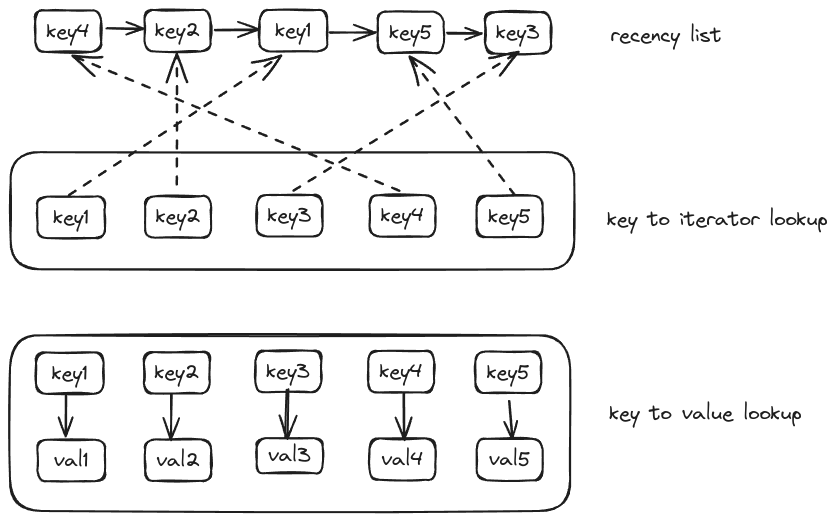
\includegraphics[width=300pt]{lru}
\end{center}

Recency list is a doubly-linked list where the most recently accessed item is at
the tail. On read or write of an existing key, the key to iterator lookup table
is used to identify the key to update. The identified key is then moved to the
tail of the recency list to indicate recent access. Finally, the key-value table
is updated if needed. When inserting a new key-value pair, the head of the
recency list is evicted to make space, if required.\\

When specifying the LRU cache with TLA+, we can omit the key to iterator table
to simplify the specification. Recency list can be implemented as a
\textit{tuple}, and a key-value table as a \textit{function}.\\

\subsection{Specification}

The following implements the LRU put function:\\

\begin{tla}
Put(k, v) == 
    IF k \in DOMAIN lru_kv THEN 
        \* replace
        /\ lru_recency' = Append(SelectSeq(lru_recency, LAMBDA x : x # k), k)
        /\ lru_kv' = [n \in DOMAIN lru_kv |-> IF n = k THEN v ELSE lru_kv[n]]
        /\ UNCHANGED lru_size
    ELSE 
        IF Len(lru_recency) # lru_size THEN 
            \* add 
            /\ lru_recency' = Append(lru_recency, k)
            /\ lru_kv' = [n \in DOMAIN lru_kv \cup {k} |-> n]
            /\ UNCHANGED lru_size
        ELSE 
            \* replace oldest 
            /\ lru_recency' = Append(SelectSeq(lru_recency,         
                                LAMBDA x : x # lru_recency[1]), k)
            /\ lru_kv' = [n \in (DOMAIN lru_kv \cup {k}) \ {lru_recency[1]} |-> 
                            IF n # k THEN lru_kv[n] ELSE v]
            /\ UNCHANGED lru_size
\end{tla}
\begin{tlatex}
\@x{ Put ( k ,\, v ) \.{\defeq}}%
\@x{ {\IF} k \.{\in} {\DOMAIN} lru\_kv \.{\THEN}}%
\@x{\@s{4.1}}%
\@y{%
  replace
}%
\@xx{}%
 \@x{\@s{4.1} \.{\land} lru\_recency \.{'} \.{=} Append ( SelectSeq (
 lru\_recency ,\, {\LAMBDA} x \.{:} x \.{\neq} k ) ,\, k )}%
 \@x{\@s{4.1} \.{\land} lru\_kv \.{'} \.{=} [ n \.{\in} {\DOMAIN} lru\_kv
 \.{\mapsto} {\IF} n \.{=} k \.{\THEN} v \.{\ELSE} lru\_kv [ n ] ]}%
\@x{\@s{4.1} \.{\land} {\UNCHANGED} lru\_size}%
\@x{ \.{\ELSE}}%
\@x{\@s{16.4} {\IF} Len ( lru\_recency ) \.{\neq} lru\_size \.{\THEN}}%
\@x{\@s{20.5}}%
\@y{%
  add 
}%
\@xx{}%
 \@x{\@s{20.5} \.{\land} lru\_recency \.{'} \.{=} Append ( lru\_recency ,\, k
 )}%
 \@x{\@s{20.5} \.{\land} lru\_kv \.{'} \.{=} [ n \.{\in} {\DOMAIN} lru\_kv
 \.{\cup} \{ k \} \.{\mapsto} n ]}%
\@x{\@s{20.5} \.{\land} {\UNCHANGED} lru\_size}%
\@x{\@s{16.4} \.{\ELSE}}%
\@x{\@s{32.8}}%
\@y{%
  replace oldest 
}%
\@xx{}%
 \@x{\@s{32.8} \.{\land} lru\_recency \.{'} \.{=} Append ( SelectSeq (
 lru\_recency ,\,}%
\@x{\@s{41.0} {\LAMBDA} x \.{:} x \.{\neq} lru\_recency [ 1 ] ) ,\, k )}%
 \@x{\@s{32.8} \.{\land} lru\_kv \.{'} \.{=} [ n \.{\in} ( {\DOMAIN} lru\_kv
 \.{\cup} \{ k \} ) \.{\,\backslash\,} \{ lru\_recency [ 1 ] \} \.{\mapsto}}%
\@x{\@s{32.8} {\IF} n \.{\neq} k \.{\THEN} lru\_kv [ n ] \.{\ELSE} v ]}%
\@x{\@s{32.8} \.{\land} {\UNCHANGED} lru\_size}%
\end{tlatex}
\\

When the implementation needs to extract a key and move it to the end, it uses
\textit{SelectSeq} to remove the targeted key and \textit{Append} to append the
key to the end. When updating \textit{lru\_kv}, the keyspace is expanded with
\textit{k}. In the case keyspace is full, then \textit{lru\_recency[1]} (least 
recent entry in LRU) is evicted.

\subsection{Safety}

For safety, we want to ensure values in \textit{lru\_recency} match with keys
in \textit{lru\_function}. Similarly, LRU size cannot exceed \textit{lru\_size}.\\

\begin{tla}
    Consistent ==
    /\ {lru_recency[k] : k \in DOMAIN lru_recency} = DOMAIN lru_kv
    /\ Cardinality(DOMAIN lru_kv) <= lru_size
\end{tla}
\begin{tlatex}
\@x{\@s{16.4} Consistent \.{\defeq}}%
 \@x{\@s{16.4} \.{\land} \{ lru\_recency [ k ] \.{:} k \.{\in} {\DOMAIN}
 lru\_recency \} \.{=} {\DOMAIN} lru\_kv}%
\@x{\@s{16.4} \.{\land} Cardinality ( {\DOMAIN} lru\_kv ) \.{\leq} lru\_size}%
\end{tlatex}

\subsection{Liveness}

Omitted from this chapter. 

\section{KV Store}

The KV store itself is pretty straightforward in design. Naively we need a
single \textit{function} to implement a table that holds the key-value pairs.
The slight complexity is integrating LRU into the KV store. This is described in
the \textit{Update} function:\\

\begin{tla}
Update(k, v) == 
    IF LRU!Contains(k) THEN 
         /\ LRU!Put(k, v)
         /\ UNCHANGED kv
         /\ latency' = CACHED
    ELSE \* LRU does not contain k
        /\ IF LRU!IsFull THEN 
                LET 
                    pair == LRU!GetLeastRecent
                    key == CHOOSE only \in DOMAIN pair: TRUE
                    value == pair[key]
                IN 
                    \* Evicted from LRU and write to memory
                    /\ kv' = [x \in DOMAIN kv \cup {key} |-> 
                                IF x = key THEN value ELSE kv[x]]
            ELSE 
                UNCHANGED kv 
        /\ LRU!Put(k, v)
        /\ latency' = EVICT
\end{tla}
\begin{tlatex}
\@x{ Update ( k ,\, v ) \.{\defeq}}%
\@x{\@s{16.4} {\IF} LRU {\bang} Contains ( k ) \.{\THEN}}%
\@x{\@s{24.59} \.{\land} LRU {\bang} Put ( k ,\, v )}%
\@x{\@s{24.59} \.{\land} {\UNCHANGED} kv}%
\@x{\@s{24.59} \.{\land} latency \.{'} \.{=} CACHED}%
\@x{\@s{16.4} \.{\ELSE}}%
\@y{%
  LRU does not contain k
}%
\@xx{}%
\@x{\@s{32.8} \.{\land} {\IF} LRU {\bang} IsFull \.{\THEN}}%
\@x{\@s{41.0} \.{\LET}}%
\@x{\@s{57.4} pair \.{\defeq} LRU {\bang} GetLeastRecent}%
 \@x{\@s{57.4} key \.{\defeq} {\CHOOSE} only \.{\in} {\DOMAIN} pair \.{:}
 {\TRUE}}%
\@x{\@s{57.4} value \.{\defeq} pair [ key ]}%
\@x{\@s{41.0} \.{\IN}}%
\@x{\@s{57.4}}%
\@y{%
  Evicted from LRU and write to memory
}%
\@xx{}%
 \@x{\@s{57.4} \.{\land} kv \.{'} \.{=} [ x \.{\in} {\DOMAIN} kv \.{\cup} \{
 key \} \.{\mapsto}}%
\@x{\@s{57.4} {\IF} x \.{=} key \.{\THEN} value \.{\ELSE} kv [ x ] ]}%
\@x{\@s{36.89} \.{\ELSE}}%
\@x{\@s{53.29} {\UNCHANGED} kv}%
\@x{\@s{32.8} \.{\land} LRU {\bang} Put ( k ,\, v )}%
\@x{\@s{32.8} \.{\land} latency \.{'} \.{=} EVICT}%
\end{tlatex}
\\

If the LRU contains the key (full or not), we simply update the LRU. The LRU will
update its internal recency list. If LRU doesn't contain the key, we have two
possible scenarios. If the LRU is not full, we can simply insert it into the LRU.
If the LRU is full, we need to evict the least recently used key-value pair 
write back to KV store, and insert the new key-value pair into the LRU.

\subsection{Safety}

Omitted from this chapter. 

\subsection{Liveness}

Omitted from this chapter. 

\section{Test}

Putting everything together, we want to characterize the design and
confirm wget get the expected latency improvement. 

\subsection{Spec}

The core of the test is pretty straightforward, we assume the usual 80/20 rule
where 80\% of the traffic are cache hits and 20\% are cache misses. This can be
simulated using the existential qualifier:\\

\begin{tla}
Next ==
    \/ \E p \in 1..10:
        /\  IF p > 2 THEN
                \* cached
                /\ \E k \in DOMAIN lru_kv:
                    /\ KV!Update(k, lru_kv[k])
                    /\ written' = [x \in DOMAIN written \ {k} |-> 
                                    IF x = k THEN k ELSE written[x]]
            ELSE 
                \* cache miss
                \* /\ PrintT(p)
                /\ \E k \in DataSet \ DOMAIN lru_kv:
                    /\ KV!Update(k, k)
                    /\ written' = [x \in DOMAIN written \ {k} |-> 
                                    IF x = k THEN k ELSE written[x]]
\end{tla}
\begin{tlatex}
\@x{ Next \.{\defeq}}%
\@x{\@s{16.4} \.{\lor} \E\, p \.{\in} 1 \.{\dotdot} 10 \.{:}}%
\@x{\@s{20.5} \.{\land}\@s{4.1} {\IF} p \.{>} 2 \.{\THEN}}%
\@x{\@s{28.7}}%
\@y{%
  cached
}%
\@xx{}%
\@x{\@s{28.7} \.{\land} \E\, k \.{\in} {\DOMAIN} lru\_kv \.{:}}%
\@x{\@s{32.8} \.{\land} KV {\bang} Update ( k ,\, lru\_kv [ k ] )}%
 \@x{\@s{32.8} \.{\land} written \.{'} \.{=} [ x \.{\in} {\DOMAIN} written
 \.{\,\backslash\,} \{ k \} \.{\mapsto}}%
\@x{\@s{36.89} {\IF} x \.{=} k \.{\THEN} k \.{\ELSE} written [ x ] ]}%
\@x{\@s{24.6} \.{\ELSE}}%
\@x{\@s{41.0}}%
\@y{%
  cache miss
}%
\@xx{}%
\@x{\@s{41.0}}%
\@y{%
  /\ PrintT(p)
}%
\@xx{}%
 \@x{\@s{41.0} \.{\land} \E\, k \.{\in} DataSet \.{\,\backslash\,} {\DOMAIN}
 lru\_kv \.{:}}%
\@x{\@s{45.1} \.{\land} KV {\bang} Update ( k ,\, k )}%
 \@x{\@s{45.1} \.{\land} written \.{'} \.{=} [ x \.{\in} {\DOMAIN} written
 \.{\,\backslash\,} \{ k \} \.{\mapsto}}%
\@x{\@s{49.19} {\IF} x \.{=} k \.{\THEN} k \.{\ELSE} written [ x ] ]}%
\end{tlatex}
\\

\subsection{Safety}

We want to verify the KV store with cache returns the correct value for 
all the key-value pairs written:\\

\begin{tla}
Consistent == 
    \A k \in DOMAIN written: 
        KV!Read(k) = written[k]
\end{tla}
\begin{tlatex}
\@x{ Consistent \.{\defeq}}%
\@x{\@s{16.4} \A\, k \.{\in} {\DOMAIN} written \.{:}}%
\@x{\@s{20.5} KV {\bang} Read ( k ) \.{=} written [ k ]}%
\end{tlatex}

\subsection{Liveness}

Omitted for this chapter.

\section{Statistical Sampling}

To collect statistical latency numbers for the design, include the Community
Module CSV and define Safety property:\\

\begin{tla}
CSVFile ==
    "stat.csv"

Stats ==
    /\ CSVWrite("%1$s", <<latency>>, CSVFile)
\end{tla}
\begin{tlatex}
\@x{ CSVFile \.{\defeq}}%
\@x{\@s{16.4}\@w{stat.csv}}%
\@pvspace{8.0pt}%
\@x{ Stats \.{\defeq}}%
 \@x{\@s{16.4} \.{\land} CSVWrite (\@w{\%1\$s} ,\, {\langle} latency {\rangle}
 ,\, CSVFile )}%
\end{tlatex}
\\

The Safety property \textit{Stats} will be triggered in every state, collecting
the latency number in a .csv. To generate the .csv: 

\begin{verbatim}
rm -rf *.csv 
    && java -cp tla2tools.jar tlc2.TLC \
        -generate -note ~/dev/tla/tla/test_kv
\end{verbatim}

The latency numbers have now been collected into stat.csv. Now let us count the
latency numbers:

\begin{verbatim}
cat stat.csv  | grep 10 -ws | wc 
    && cat stat.csv  | grep 100 -ws | wc

  34674   34674  104022
   9239    9239   36956
\end{verbatim}

With a total of 43913 samples, cache hit happens about 78.9\% of the time. This 
closely matches the desired 80\% cache hit defined in the test.

% \end{document}
